\documentclass[a4]{article}
\usepackage{amssymb}
\usepackage{amsmath}
\usepackage{listings}
\usepackage{graphicx}
\usepackage{../../manual/manual}
\newcounter{lst}[section]

\renewcommand{\thelst}{\arabic{section}.\arabic{lst}}

\lstset{basicstyle=\footnotesize\sffamily}

\lstdefinestyle{easslisting}{basicstyle=\footnotesize\sffamily, mathescape=true, frame=tb,  numbers=right, numberstyle=\footnotesize, stepnumber=1, numbersep=-5pt, captionpos=b}

\lstdefinestyle{eass}{basicstyle=\sffamily, mathescape=true}

\lstnewenvironment{listing}[3]{
  \noindent        
  \refstepcounter{lst}         
  \label{code:#1}  
\begin{tabular}{p{.97\columnwidth}} \\ \hline  {\normalsize \textbf{Code  fragment \arabic{section}.\arabic{lst}} #2} \\  \end{tabular} 
\lstset{language=#3,          
  basicstyle=\footnotesize\sffamily,
%%%  basicstyle=\footnotesize,    
  xleftmargin=10pt,    
  mathescape=true,    
  frame=tb,    
  numbers=right,    
%%%  numberstyle=\tiny,     
  numberstyle=\footnotesize,     
  stepnumber=1,     
  numbersep=-5pt}}{}

%-- definition for Gwendolen --%

\lstdefinelanguage{Gwendolen}{%
    morekeywords={Plans,Initial,Beliefs,Goals,name,fof-parse,Rules,Belief,Reasoning},
    morecomment=[l]{//},
 literate= {<-}{{$\leftarrow$}{$\:$}}2
           {.B}{{${\cal B}$}}2
           {.G}{{${\cal G}$}}2
           {lnot}{{$\sim$}}2
           {assert_shared}{{$+_{\Sigma}$}}2
           {remove_shared}{{$-_{\Sigma}$}}2
           {(perform)}{}0
}



\makeindex

\author{Louise A. Dennis}

\title{\eass\ Tutorial 1 -- Comparison with \gwendolen}

\begin{document}
\maketitle
This is the first in a series of tutorials on the use of the \eass\ variant of the \gwendolen\ language that was first developed as part of the Engineering Autonomous Space Software project.  The \eass\ variant is adapted for use with physical systems and simulations, such as mobile robots, satellites and unmanned aircraft.  This tutorial covers the basic concepts behind the \eass\ variant and its differences to the \gwendolen\ language.  

Files for this tutorial can be found in the \texttt{mcapl} distribution in the directory \texttt{src/examples/eass/tutorials/tutorial1}.

The tutorial assumes familiarity with the \gwendolen\ programming language.

\section{Abstraction and Reasoning Engines}

\begin{figure}[htb]
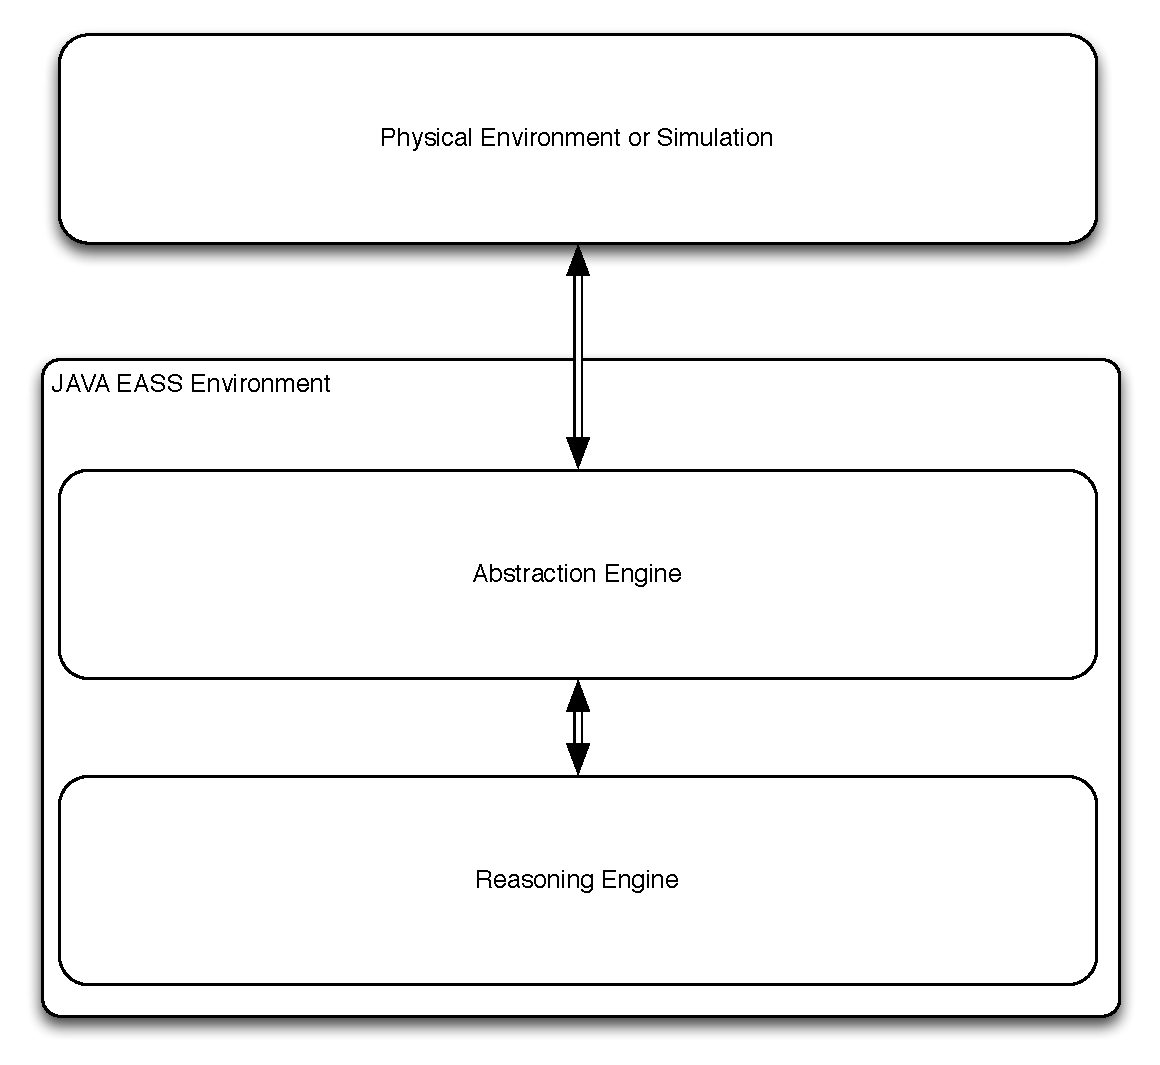
\includegraphics[width=\textwidth]{arch.pdf}
\caption{The Architecture of an \eass\ Agent}
\label{fig:arch}
\end{figure}
Figure~\ref{fig:arch} shows the architecture of an \eass\ Agent.  The agent is actually a pair of agents, the \emph{reasoning engine} which is responsible for complicated reasoning tasks, and the \emph{abstraction engine} which is responsible for processing and filtering incoming perceptions so only those actually needed for reasoning are passed on to the reasoning engine itself.

The reasons for this separation are primarily driven by the observation that BDI agents are unable to process incoming perceptions from real or simulated sources fast enough and so they get ``clogged'' by an ever increasing number of intentions to do with perception processing.  

The theoretical underpinnings of this architecture are described in~\cite{DALT10:abstraction}.  The key points are that the \emph{reasoning engine} does not interact with the physical world (or a simulation) at all.  It gains perceptions via \emph{shared beliefs} which are communicated with the abstraction engine via the Java \eass\ environment.  Similarly most of its actions (ideally all) are communicated to the abstraction engine which then reifies them (e.g., adding more low level detail that may be required by the physical system or simulation to actually enact the action.  As a rule of thumb while perceptions and actions, as used by the physical system or simulation generally involve numeric values, reasoning generally uses logical (``yes/no'') information and outputs simple non-numeric commands.  Therefore the abstraction engine should be responsible for converting numeric data (``distance = 5.4m'') into logical statements (``too close'') and converting simple commands (``slow down'') into numerical instructions (``apply a decelleration of $-1m/s^2$'').  This is only a rule of thumb and the reality is that a certain amount of experimentation is often required to balance a system appropriately so that reasoning happens fast enough to adequately control the physical system.

In order for this to work \gwendolen's reasoning cycle was adapted slightly, a set of dedicated actions were introduced for handling shared beliefs and delegated actions, and some new constructs were added to the language.

\section{Key Differences}
\subsection{Perception Processing}
In the \gwendolen\ language incoming perceptions are converted into intentions which contains a deed to add the perception to the belief base.  In theory this gives the agent more control over the contents of its beliefs (although in practice no use has ever been made of this).  However a side effect is that it take the agent two turns of the reasoning cycle to convert a perception into a belief and this slowed down the processing of perceptions.

In the \eass\ variant, therefore, new perceptions are placed directly into the agent's belief base during the perception stage of the reasoning cycle.

\subsection{Abstraction Engines}
Since each agent is, in fact, a pair of agents, it is necessary to identify and link 


\bibliographystyle{abbrv} %% {plain}
\bibliography{../../manual/manual}

\end{document}
